%% ----------------------------------------------------------------
%% GDP.tex
%% ---------------------------------------------------------------- 
\documentclass{ecsdocs/ecsgdp}         % Use the GDP Report Style
\graphicspath{{../Figures/}}   % Location of your graphics files
\usepackage{natbib}            % Use Natbib style for the refs.
\usepackage{array}
\usepackage{lscape}
\usepackage{enumitem}       % For making numbered indent lists
\hypersetup{colorlinks=true}   % Set to false for black/white printing
%%% ----------------------------------------------------------------
%% Definitions.tex
%% ---------------------------------------------------------------- 
\newcommand{\BibTeX}{{\rm B\kern-.05em{\sc i\kern-.025em b}\kern-.08em T\kern-.1667em\lower.7ex\hbox{E}\kern-.125emX}}

%% People
\newcounter{address}
\setcounter{address}{1}
\renewcommand{\theaddress}{\textsuperscript{\fnsymbol{address}}}
\newcommand{\address}[1]{\refstepcounter{address}\theaddress#1\\}
\newcommand{\Name}[3]{\texorpdfstring{\href{mailto:#3}{#2}#1}{#2}\xspace}
\newcommand{\SteveRGunn}[1]{\Name{#1}{Steve R. Gunn}{S.R.Gunn@ecs.soton.ac.uk}}

%% Dingbats
\newcommand{\tick}{\ding{51}}
\newcommand{\cross}{\ding{55}}

%% Calculus
\newcommand{\pd}[2]{\ensuremath{\frac{\partial #1}{\partial #2}}\xspace}
\newcommand{\fd}[2]{\ensuremath{\frac{d #1}{d #2}}\xspace}
\newcommand{\dint}{\ensuremath{\int\!\!\!\int}\xspace}
\newcommand{\tint}{\ensuremath{\int\!\!\!\int\!\!\!\int}\xspace}

%% Math Sets
\newcommand{\Q}[1]{\ensuremath{\mathbb{#1}}\xspace}
\newcommand{\R}{\Q{R}}

%% Matrix, Vector
\newcommand{\V}[1]{\ensuremath{\boldsymbol{#1}}\xspace}
\newcommand{\M}[1]{\ensuremath{\boldsymbol{#1}}\xspace}
\newcommand{\0}{\V{0}}
\newcommand{\1}{\V{1}}
\newcommand{\I}{\M{I}}

%% Math Functions
\newcommand{\F}[1]{\ensuremath{\mathrm{#1}}\xspace}
\newcommand{\sgn}{\F{sgn}}
\newcommand{\tr}{\F{trace}}
\newcommand{\diag}{\F{diag}}

%% Math Names
\newcommand{\N}[1]{\ensuremath{\mathit{#1}}\xspace}

%% Data
\newcommand{\mc}[1]{\ensuremath{\mathcal{#1}}\xspace}
\newcommand{\Hyp}{\mc{H}}
\newcommand{\D}{\mc{D}}

%% Kernel
\newcommand{\K}{\M{K}}
\newcommand{\eins}{\texorpdfstring{\ensuremath{\epsilon}}{\textepsilon}-insensitive\xspace}
\newcommand{\e}{\ensuremath{\epsilon}\xspace}
\newcommand{\Bxi}{\ensuremath{\boldsymbol{\xi}}\xspace}
\newcommand{\Kanova}{\ensuremath{\mathit{K_{ANOVA}}}\xspace}
\newcommand{\Kspline}{\ensuremath{\mathit{K_{spline}}}\xspace}

%% Bayesian
\newcommand{\MP}{\ensuremath{\mathit{{\scriptscriptstyle \hspace{-1.5pt}M\hspace{-1.5pt}P}}}\xspace}
\newcommand{\ML}{\ensuremath{\mathit{{\scriptscriptstyle \hspace{-1.5pt}M\hspace{-1.5pt}L}}}\xspace}
\newcommand{\Qw}{\ensuremath{Q_{\w}(\w)}\xspace}
\newcommand{\Qa}{\ensuremath{Q_{\Ba}(\Ba)}\xspace}
\newcommand{\Qb}{\ensuremath{Q_{\beta}(\beta)}\xspace}
\newcommand{\wMPab}{\ensuremath{\w_{\MP|\bar {\Ba},\bar \beta}}\xspace}
\newcommand{\wMP}{\ensuremath{\w_{\MP}}\xspace}
\newcommand{\yMP}{\ensuremath{y_{\MP}}\xspace}
\newcommand{\BaMP}{\ensuremath{\Ba_{\hspace{1pt}\MP}}\xspace}
\newcommand{\aMP}{\ensuremath{\alpha_{\hspace{1pt}\MP}}\xspace}
\newcommand{\bMP}{\ensuremath{\beta_{\hspace{1pt}\MP}}\xspace}
\newcommand{\Sab}{\ensuremath{\M{\Sigma}_{\bar \Ba,\bar \beta}}\xspace}
\newcommand{\Ba}{\ensuremath{\boldsymbol{\alpha}}\xspace}
\newcommand{\Bb}{\ensuremath{\boldsymbol{\beta}}\xspace}
\newcommand{\Bm}{\ensuremath{\boldsymbol{\mu}}\xspace}
\newcommand{\BL}{\ensuremath{\boldsymbol{\Lambda}}\xspace}
\newcommand{\BPhi}{\ensuremath{\boldsymbol{\Phi}}\xspace}
\newcommand{\SMP}{\ensuremath{\M{\Sigma}_{\MP}}\xspace}

\newcommand{\Pa}{\ensuremath{P(\alpha|\mathcal{H})}\xspace}
\newcommand{\Pb}{\ensuremath{P(\beta|\mathcal{H})}\xspace}
\newcommand{\Pab}{\ensuremath{P(\alpha,\beta|\mathcal{H})}\xspace}
\newcommand{\Pw}{\ensuremath{P(\w|\mathcal{H})}\xspace}
\newcommand{\PD}{\ensuremath{P(\D|\mathcal{H})}\xspace}
\newcommand{\PwIa}{\ensuremath{P(\w|\alpha,\mathcal{H})}\xspace}
\newcommand{\PDIwb}{\ensuremath{P(\D|\w,\beta,\mathcal{H})}\xspace}
\newcommand{\PDwab}{\ensuremath{P(\D,\w,\alpha,\beta|\mathcal{H})}\xspace}
\newcommand{\PDIw}{\ensuremath{P(\D|\w,\mathcal{H})}\xspace}
\newcommand{\PwID}{\ensuremath{P(\w|\D,\mathcal{H})}\xspace}
\newcommand{\PwabID}{\ensuremath{P(\w,\alpha,\beta|\D,\mathcal{H})}\xspace}

\newcommand{\PanH}{\ensuremath{P(\alpha)}\xspace}
\newcommand{\PbnH}{\ensuremath{P(\beta)}\xspace}
\newcommand{\PabnH}{\ensuremath{P(\alpha,\beta)}\xspace}
\newcommand{\PwnH}{\ensuremath{P(\w)}\xspace}
\newcommand{\PDnH}{\ensuremath{P(\D)}\xspace}
\newcommand{\PwIanH}{\ensuremath{P(\w|\alpha)}\xspace}
\newcommand{\PDIwbnH}{\ensuremath{P(\D|\w,\beta)}\xspace}
\newcommand{\PDwabnH}{\ensuremath{P(\D,\w,\Ba,\beta)}\xspace}
\newcommand{\PDIwnH}{\ensuremath{P(\D|\w)}\xspace}
\newcommand{\PwIDnH}{\ensuremath{P(\w|\D)}\xspace}
\newcommand{\PwabIDnH}{\ensuremath{P(\w,\alpha,\beta|\D)}\xspace}

\newcommand{\PDwBab}{\ensuremath{P(\D,\w,\Ba,\beta|\mathcal{H})}\xspace}
\newcommand{\PwIBa}{\ensuremath{P(\w|\Ba,\mathcal{H})}\xspace}
\newcommand{\PBab}{\ensuremath{P(\Ba,\beta|\mathcal{H})}\xspace}
\newcommand{\PwBabID}{\ensuremath{P(\w,\Ba,\beta|\D,\mathcal{H})}\xspace}

\newcommand{\PBanH}{\ensuremath{P(\Ba)}\xspace}
\newcommand{\PwIBanH}{\ensuremath{P(\w|\Ba)}\xspace}

%% Snakes
\newcommand{\Esnake}{\ensuremath{\mathit{E_{snake}}}\xspace}
\newcommand{\Eimage}{\ensuremath{\mathit{E_{image}}}\xspace}
\newcommand{\Econt}{\ensuremath{\mathit{E_{cont}}}\xspace}
\newcommand{\Ecurv}{\ensuremath{\mathit{E_{curv}}}\xspace}
\newcommand{\Eint}{\ensuremath{\mathit{E_{int}}}\xspace}
\newcommand{\Eext}{\ensuremath{\mathit{E_{ext}}}\xspace}
\newcommand{\Eterm}{\ensuremath{\mathit{E_{term}}}\xspace}
\newcommand{\Eline}{\ensuremath{\mathit{E_{line}}}\xspace}
\newcommand{\Eedge}{\ensuremath{\mathit{E_{edge}}}\xspace}
\newcommand{\Econ}{\ensuremath{\mathit{E_{con}}}\xspace}
\newcommand{\Eangle}{\ensuremath{\mathit{E_{angle}}}\xspace}
\newcommand{\Elshape}{\ensuremath{\mathit{E_{lshape}}}\xspace}
\newcommand{\Eedgedir}{\ensuremath{\mathit{E_{edgedir}}}\xspace}
\newcommand{\Emodel}{\ensuremath{\mathit{E_{model}}}\xspace}
\newcommand{\wte}{\ensuremath{\mathit{w_{term}}}\xspace}
\newcommand{\wli}{\ensuremath{\mathit{w_{line}}}\xspace}
\newcommand{\wed}{\ensuremath{\mathit{w_{edge}}}\xspace}
\newcommand{\wco}{\ensuremath{\mathit{w_{con}}}\xspace}

%% Environments
\newcounter{alg}
\newenvironment{algorithm}[1]
{
    \stepcounter{alg}
    \begin{table}[htb]
    \centering
    \begin{tabular}[t]{ll}
    \hline&\\
    \multicolumn{2}{l}{\bf Algorithm \arabic{alg}: #1}\\&\\
} {
    &\\
    \hline
    \end{tabular}
    \end{table}
}
            % Include your abbreviations
%% ----------------------------------------------------------------
\begin{document}
	\frontmatter
	\title{TEST TITLE}
	\authors    {\texorpdfstring
		{\href{mailto:S.R.Gunn@ecs.soton.ac.uk}{Steve R. Gunn}}
		{Steve R. Gunn}
	}
	\addresses  {\groupname\\\deptname\\\univname}
	\date       {\today}
	\subject    {}
	\keywords   {}
	\supervisor{Dr. Geoff Merrett \\ Dr. Alex Weddell}
	\examiner{Dr. Klaus-Peter Zauner}
	\degree     {Master of Engineering}
	\maketitle
	\begin{abstract}
		This work is all about \dots
	\end{abstract}
	\tableofcontents
	\listoffigures
	\listoftables
	\lstlistoflistings
	\listofsymbols{ll}{$w$ & The weight vector}
	%\acknowledgements{Thanks to no one.}
	%\dedicatory{To \dots}
	\mainmatter
	%% ----------------------------------------------------------------
	% Introduction chapter
	\chapter{Introduction}

Ultra-Low Power Processors, such as ARM's Cortex-M0+, are becoming an increasingly appealing area of research, particularly because they provide a platform for the Internet of Things. As our culture develops new ways for technology to aid our every-day lives, the devices which support these progressions are required to be less and less intrusive, forcing companies to search for new methods of making systems smaller and require lower power, especially as ``essentially all IoT sensor nodes will be powered by small batteries and to a lesser extent by energy harvesting'' \cite{iot_power}.

However, such processors clearly create very tight constraints for potential developers, as processing power is often limited, leading to the ever-continuing requirement for more efficient and optimised algorithms. As memory usage is also proportional to power consumption, the RAM available on such systems is extremely limiting. As we begin to rely on these systems more and more, these constraints make it a growing challenge to implement systems which are not only useful, but can be relied upon to function when needed. This is particularly important in cases in which a device is being used for safety-critical operations, which is becoming increasingly common \cite{iot_saftey} \cite{iot_saftey2}.

ARM is currently investigating the concept of a sub threshold Cortex-M0+ \cite{arm_sub}, which attempts to push the extremes of these constraints further by providing just 8 kB of memory for both program code and data, and running at just a few hundred kHz. This project aims to research and develop an algorithm which is capable of running on such a device, to act as a proof of concept that such a processor would be worthwhile.

\namedsection{Project Overview}{Finch}

The particular algorithm that the group developed is a way to identify and monitor exercises performed by a human wearer. These are specifically exercises which can be done on aeroplanes to reduce the risk of suffering from Deep Vein Thrombosis, a condition where a blood clot can form in one of the deep veins in the body, most commonly the legs. This can lead to further complications such as pulmonary embolism which occurs when part of the blood clot moves and blocks a blood vessel in the lungs \cite{dvt}. Long-haul flights can increase the risk of getting DVT because of the long periods of time sitting down and not moving which reduces circulation in the legs.

\begin{figure}[h]
  \centering
    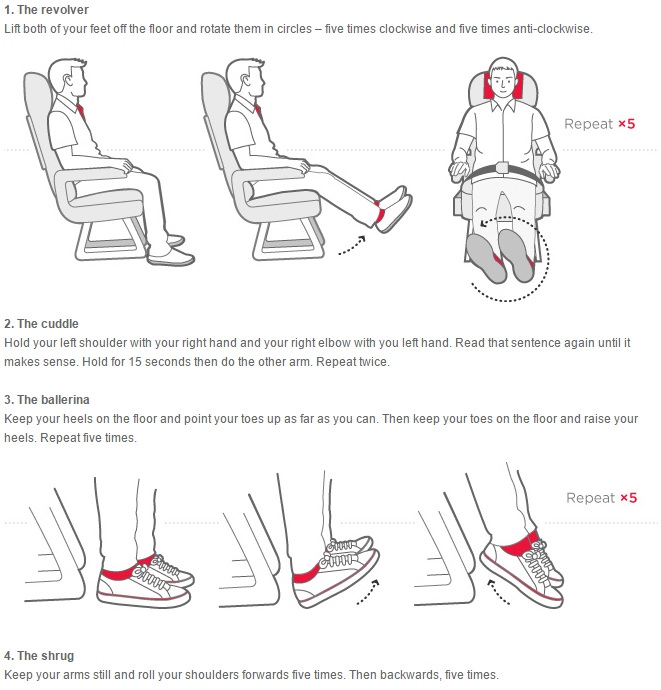
\includegraphics[width=1.0\textwidth]{figures/exercises}
  \caption{In-flight exercises \cite{virgin2015exercises}}
  \label{fig:exercises}
\end{figure}

Figure \ref{fig:exercises} shows some of the in-flight exercises which can be performed. A few of them were looked into including the revolver, the ballerina and the shrug. These involve lifting both feet off the floor and rotating them in circles in clockwise and anticlockwise directions, pointing the feet up and down and rolling the shoulders backwards and forwards. These are all designed to help keep the circulation going in the limbs. However, a specific focus was made to the revolver exercise for the purpose of prototyping a system.

Possible uses of the algorithm would be to incorporate it into a device which could be given to passengers to strap to their legs. It would then monitor how much exercise each person was doing. This could help inform the passengers whether or not they are doing enough exercise to stay risk free. The device itself could make use of energy efficient technologies (for example the Cortex-M0+) so that its battery could easily last the entire duration of a long-haul fight.

\namedsection{Project Requirements }{Finch}

The main requirement of this project is to develop an algorithm which is capable of detecting and monitoring exercises on a sub threshold Cortex-M0+. This processor is clocked at 100 kHz, although it can increase to 3 MHz if required. However, the lower the clock speed the better as this would clearly require less power.

Additionally, 8 kB is imposed as the memory limit for both program code and data in order for the algorithm to be capable of running on the sub threshold Cortex-M0+. Again, the lower this can be the better as it opens up the possibility for the system to require even less power.

As the proposed sub threshold Cortex-M0+ is still in development, it is not readily available for the group to use; consequently, the team was required to investigate alternatives to emulate the processor. These alternatives must allow the clock speeds to be adjusted based on the efficiency and requirements of the algorithm. The challenges involved in this are discussed in chapter~\ref{chap:embedded}.

Research and analysis of the algorithms used for exercise detection which currently exist, specifically focusing on Machine Learning techniques, was also carried out. On top of this, an investigation into the tools and techniques which can be used, along with the methods by which the effectiveness of trained algorithms can be evaluated was also necessary. This is documented in chapter~\ref{chap:research}.

Following on from this, the ways in which the algorithm can be optimised to run on a such constrained system must also be explored. The way this was done is examined in chapter~\ref{chap:software}.

Another requirement of the project was to perform a user study to collect movement data of the exercises which can be used to develop the algorithm. This is so that a range of data from a selection of different people can be used because each individual is likely to perform the exercises with slight variations. The details of this can be found in chapter~\ref{chap:study}.

Finally, the accuracy of the developed algorithm is calculated; the specifics of this are outlined in chapter~\ref{chap:results}.
Below, the requirements of this project are given in explicit detail.

\namedsection{Detailed Requirements}{Finch}

\begin{enumerate}
  \item The algorithm must be capable of detecting and monitoring exercises designed to combat deep vein thrombosis
  \begin{enumerate}[label*=\arabic*.]
    \item These are exercises which can be performed in a plane, particularly in long haul flights and include:
    \begin{enumerate}[label*=\arabic*.]
      \item Foot rotations
      \item Pointing feet up and down
      \item Shoulder rolling
    \end{enumerate}
    \item Other activities such as walking should be distinguished as not being exercise
  \end{enumerate}
  \item The algorithm must be suitable to execute on an ultra-low-power sub threshold ARM Cortex-M0+
  \begin{enumerate}[label*=\arabic*.]
    \item This device has a limited processor clocked from 100 kHz to a maximum of 3 MHz
    \item Memory usage should be kept to a minimum with a target of no more than 8 kB
    \item Therefore, the algorithm should be highly optimised to use as little memory and require as little processing power as possible
  \end{enumerate}
  \item The sub threshold Cortex-M0+ must be emulated in a test platform as working with the actual M0+ is not feasible
  \begin{enumerate}[label*=\arabic*.]
    \item The test platform should be capable of being clocked at frequencies ranging from only a 100 kHz to 3 MHz
    \item The test platform should have at least 32 kB of memory to aid with testing and to act as a fall back if 8 kB cannot be achieved
    \item There must be an accelerometer sensor on the platform that readings can be taken from
  \end{enumerate}
  \item Research into various potential algorithms must take place
  \begin{enumerate}[label*=\arabic*.]
    \item Machine learning approaches should be focussed on
    \item Algorithms which are used on unconstrained systems should be considered first
    \item The feasibility of constraining those algorithms should then be investigated
    \item The methods of evaluating algorithm performance should also be examined
  \end{enumerate}
  \item Participant studies should be performed to gather movement data to train the algorithm
  \begin{enumerate}[label*=\arabic*.]
    \item Ethics approval will need to be obtained
  \end{enumerate}
  \item The developed algorithm must be deployed to the test platform
  \item The final system must then be evaluated in terms of its accuracy at detecting exercises
\end{enumerate}

	
	% Software chapter
	\chapter{Software Development}\label{chap:software}

We have discussed the requirements of the chosen algorithm, and had a detailed overview of the capabilities and limitations of the hardware available to the team. This chapter gives analysis of the tools and techniques used to develop such an algorithm, and discusses some of the trade-offs and optimisations that were investigated.

\namedsection{Developing the Algorithm}{Shepherd}

Taking into account the constraints of the system, we decided to focus on the MultiLayer Perceptron as it does not require matrix maths and typically has a smaller network of nodes. This session discusses the process by which we developed an implementation of this algorithm.

\subsection{Existing Weka Implementation}

As Weka had been used to determine and train the best algorithm, it was decided to inspect its source code to obtain a starting point for the algorithm development. This, while provided a good insight into the manar in which the algorithm functions, highlighted some key areas of inefficiencies that would have to be avoided when working on a subthreshold device.

\subsubsection{Backwards Propogation}

Weka's implementation of the MultiLayer Perceptron uses ``backwards propogration'', which recursively workings backwards in a depth-first mannar from each output node towards the input layer. The function which calculates a node's output does so by taking the summation of each of its input values multiplied by their respective input weights. Each input value, however, is requested on the fly from the inputting node by calculating its output which in turn causes it to perform the same loop over its input nodes:

\begin{lstlisting}[language=Java,caption={Weka's method of calculating a node's output}]
class Node
{
    double weights[NUM_INPUTS];
    Node inputs[NUM_INPUTS];
    double baseValue;

    double output()
    {
        double out = base;

        for (int i = 0; i < NUM_INPUTS; i++)
        {
            out += weights[i] * inputs[i].output();
        }

        return out;
    }
}
\end{lstlisting}

A side effect of this is that all nodes, other than the output nodes are visted multiple times. For example, for the network below, $o_1.output()$ will loop over $m_1$, $m_2$ and $m_3$, calling \verb|output()| on each, each of which will loop over $i_1$, $i_2$ and $i_3$, meaning the input nodes will be visted a total of 3 times each. This process must then be repeated for $o_2$, causing the middle layer nodes to each be revisted, and the input layers revisted another 3 times, and again for $o_3$. In total the input nodes is accessed 9 times each, the middle layer 3 times each.

\begin{figure}[!h]
    \centering
    \includegraphics{eg-ml}
    \caption{Example MultiLayer Perceptron Network}
    \label{fig:eg-ml}
\end{figure}

Weka reduces this by storing a node's value after an \verb|output()| call. When \verb|output()| is called on a node again, it checks if it has already been called and returns the cached value if it has:

\begin{lstlisting}[language=Java,caption={Weka's method of preventing repeated calculations}]
class Node
{
    boolean visited = false;
    double value;

    double output()
    {
        if (this.visited) return this.value;

        // Otherwise perform recursive calculation above

        this.visited = true;
        return this.value = out;
    }
}
\end{lstlisting}

While this does succeed in reducing the number of unnessisarry node vistits, it does not eliminiate them; each node in the network, other than the output nodes, are visited three times each with this immplementaiton. This scheme also adds two new node properties which must be stored and manipulated; the side effect of this is an increase in instructutions and memory requirement, which is not ideal for subthreshold development.

The algorithm itself still relies on recursion - this is also suboptimal as this requires extensive use of the stack.

\subsubsection{The Alternative: Forwards Propogation}

As a result of the inherant inefficiencies in a Backwards Propogation implementation, it was decided instead to redesign the algorithm, employing Forwards Propogation. This technique, in contrast to the one described above, starts from the input layer nodes and works forward in a width first mannar.

For the example in Figure \ref{fig:eg-ml}, this means the algorithm would first write the outputs of $i_1$, $i_2$ and $i_3$ into three memory spaces. Following this, three new memory spaces are reserved, in which the base values of $m_1$, $m_2$ and $m_3$ are placed. The algorithm then loops over the input nodes and, for each one, adds the multiplication of its value by its parent weight to the parent's memory space. Once complete, the outputs for all three middle layer nodes have been completed so the process can be shifted one layer to the right and repeated. An added benefit here is that the input layers are now no longer required, so their memory can be freed and reused if desired.

This method requires no stack usage and can operate in a small memory space, the equation for which is given below. For our algorithm, which has the same number of layers as the example above, this results in only 5 32bit memory spaces: 20 bytes.

\begin{equation}
\label{eq:algo-size}
\max\{\forall L_n \in LAYERS \wedge L_{n+1} \in LAYERS : |L_n|+|L_{n+1}|\}
\end{equation}

\subsection{Moving to C Code}

Weka is a very useful tool for generating and training machine learning algorithms. Unfortuneately, it only allows exporting to \verb|.model| files, which are simply Java serialized objects. As such, we were forced to modify the Weka source code in order to obtain the number, structure and weightings of the nodes in the MLP's neural network.

Once the algorithm was designed, it was decided to modify and improve the Java code such that it became a harness for our C code. In this mannar, rather than simply outputting the node structure which would have to be manually copied and amended to go into the C implementation, the Java code was built to process the nodes prior to output, removing unused layers and returning the required data in a format and structure which could be immediately compiled into the C development repository.

This proved very useful, as training the networks and trying various settings took time and was repeated many times during development. Using this harness allowed the team to quickly deploy updated models onto the device without the need to reprogram the C code for each test.
\namedsection{Developing for a Limited Environment}{Shepherd}
% This section talks about the C development

The Multilayer Perceptron is a good fit for a subthreshold Cortex M0+ as it does not require a great deal of complex mathematical computation. Unfortunately, however, it does require the use of decimal numbers and uses the sigmoid function, which requires division and power operations. This section discusses some of the design decisions and sacrifices that were made in order to implement an MLP on such a constrained system.

\subsection{Sigmoid Function}
The sigmoid function is applied to each node's output, after the summation of its weighted inputs is calculated, as discussed above in section \ref{sec:weka-code}; its graph and equation is shown below in figure \ref{fig:sigmoid}. Clearly, this equation causes two issues for the proposed device: firstly, it requires division, and secondly it requires the use of the constant \verb|e|, which is a non-integer; using this in an operation involving powers could potentially prove expensive.

The first area of note in this graph is that the value of $f(t)$ quickly starts to tend towards 0 in the negative direction, and 1 in the positive direction. It is not uncommon, therefore, to approximate the value of the function at these extremes \cite{sigmoid_approx}. Figure \ref{fig:sigmoid-ends} shows this approximation highlighted in bold for \verb|t| values outside of the range between 5 and -5; it is plain to see that the error introduced here is minimal.

\begin{figure}
    \centering
    \subfigure[Normal Sigmoid Function]{\label{fig:sigmoid}\includegraphics[width=70mm]{figures/sigmoid.pdf}}
    \subfigure[Approximated Ends]{\label{fig:sigmoid-ends}\includegraphics[width=70mm]{figures/sigmoid-ends.pdf}}
    \subfigure[Approximated With Lines]{\label{fig:sigmoid-soft}\includegraphics[width=70mm]{figures/sigmoid-soft.pdf}}
    \subfigure[Approximated With Linear Equation]{\label{fig:sigmoid-hard}\includegraphics[width=70mm]{figures/sigmoid-hard.pdf}}
    \caption{Sigmoid Functions \label{fig:sigmoid-options}}
\end{figure}

For the remaining range, between 5 and -5, the sigmoid function does not tend to any fixed value, so a different approximation must be used. Fortunately, the sigmoid's ``S''-like shape lends itself to being easily split into a series of smaller lines, as shown in figure \ref{fig:sigmoid-soft}. This provides a suitable level of accuracy with far lower computing overhead as each line can be defined using only a linear equation. However, as beneficial as the approximation in figure \ref{fig:sigmoid-soft} is, it is possible to approximate this further: using a single linear equation. This is shown in this section's final figure: \ref{fig:sigmoid-hard}. When run on the training dataset, which under non-constrained conditions achieves 94.5\% accuracy, this approximation only yields an observed drop of 3\%. This margin of error is acceptable as it can be dealt with by the added heuristics, as discussed in section \ref{sec:heuristics-alternative} above.

\subsection{Floating point \label{sec:floating-point}}
The lack of floating point support in the proposed device created a large challenge, as the neural network is entirely based upon a series of non-integer input weights, and the ability for each node to produce non integer output values. As mentioned in section \ref{sec:cortex-limitations}, the device does not have native support for hardware floating point, and floating point libraries give too much overhead to be feasible for this project. In order to get around this problem, the team opted for a fixed-point implementation: the weights of each node are multiplied by a scale factor and the resulting integer part is taken as the value.

This form is convenient as it makes the multiplication and addition of such scaled values straightforward: for addition of values using the same scale factor, it is sufficient to simply add the integers as though they were normal. The equation below illustrates this:

\begin{equation}
\label{eq:bits:addition}
x*S+y*S=(x+y)*S
\end{equation}

For the case of multiplication, the scale factors of each number must also be multiplied, meaning that when two numbers with a scale factor of $S$ are multiplied, the resulting number's scale factor is $S^2$:

\begin{equation}
\label{eq:bits:multiplication}
(x*S)(y*S)=(x*y)*S^2
\end{equation}

This can be easily rectified by simplifying dividing the result by $S$ again to return to the original scale factor:

\begin{equation}
\label{eq:bits:rescale}
\frac{(x*y)*S^2}{S}=(x*y)*S
\end{equation}

As division is not supported on our system, we have defined our scale factor $S$ as a power of 2: $S=2^B$. We are then able to approximate divisions of powers of 2, by simply performing a bit shift:

\begin{equation}
\label{eq:bits:div_approx}
X/2^B\approx X \gg B
\end{equation}

\subsubsection{Using this on the Device}

To decide the bit scale factor, $B$, for the exercise detection algorithm, it is important to consider the memory restrictions on variable size. At a hardware level, 32bits, or 4 bytes, is the maximum size an integer can be. As the algorithm requires the multiplication of numbers, ideally these would need to fit into just a 2 bytes space, as the multiplication of numbers results in the addition of powers, as shown in equation \ref{eq:bits:multiplication-shift}.

\begin{equation}
\label{eq:bits:multiplication-shift}
(x*2^B)(y*2^B)=(x*y)*(2^B)^2=(x*y)*2^{2B}
\end{equation}

As such, the value of $B$ has to be high enough such that precision is not lost unnecessarily, but low enough such that $|x*2^B|<2^{16}$. To solve this, the highest possible floating point value must be known; in the case of the algorithm, this is the base value of the first node in the middle layer: -10.6 (3s.f.); this was obtained from the training, as discussed in section \ref{ml}. Using this value in the rearranged equation, \ref{eq:bits:number-calc}, gives a bit shift of 12.

\begin{equation}
\label{eq:bits:number-calc}
B<\lfloor\log_{2}\left\{\frac{2^{16}}{|x|}\right\}\rfloor
\end{equation}

\subsubsection{Dealing with signed integers \label{sec:asr}}

The process of using simple bit shifts to act as a scale factor is acceptable if all values are known to be positive, and are as such stored unsigned. However, as the algorithm makes use of negative weights, and the gyroscope is capable of producing negative readings, the numbers used in the team's implementation are required to be signed.

Signed numbers treat the highest bit of an integer as negative, and the remaining bits as positive. This effectively shifts the range of values is able to hold, down by 50\%. Performing a naive bit shift on a negative number in this format would drastically corrupt its value by unsetting the MSB incorrectly.

For example, a value of $-10$ would be encoded as $11110110$ if stored as a signed byte. In the method described in the sections above, a bit shift to the right by 1 would be used to roughly equate to a division of $-5$, which is encoded as $11111011$. Unfortunately, this is \textit{not} the result of such a shift on $-10$; instead this shifted becomes $01111011$ which is $123$. The error has been introduced as a zero has been added into the MSB, as is convention with logical right shifts.

To avoid this, many processors, including the Cortex M0, contain an instruction known as an `Arithmetic Shift Right' (ASR) which, instead of adding a zero into the place of the MSB, it leaves whatever value was in that bit, as well as copying it to the right to perform the shift. As a result of this, positive numbers remain positive and negative numbers remain negative.

While the team's emulation platform, the Cortex M0, contains support for the ASR operation, it was unknown if the sub-threshold device would do so. As such, it was decided to implement a software alternative to support this operation, should the underlying hardware not be capable. This is shown in listing \ref{lst:asr} and can be turned on by passing \verb|-DNO_ASR| when compiling, otherwise a regular shift is used.

\begin{lstlisting}[caption={Software Arithmetic Shift Right Support},label={lst:asr}]
static void asr(int32_t val, uint8_t shift)
{
    int32_t msb = val & 0x80;     // Store the value of just the MSB

    return (val >> shift) | msb;  // Shift right then restore the MSB
}
\end{lstlisting}
\namedsection{Space Restrictions \label{sec:space-restrictions}}{Shepherd}

As described in \ref{section}\todo{REF}, the device has very little memory space availiable: 8kB for both program code and data. When the algorithm code was first compiled with the mBed's precompiled libraries, the total size of the binary was 12kB. The first step to solve this was to obtain the source code for the mBed libraries; compiling these directly along with the program code, offers further potencial for the compiler to optimise the link between the API and the algorithm, based on the specific usecase.

The method was successful at reducing the total binary size to 8kB. This was a substancial improvement, however it was clear that this would need to be decreased further as an 8kB binary leaves no room for heap or stack space when the code is run.

\subsection{Improving GCC's Optimisations}

While ARM's compiler is very good at optimising code when it compiles C and C++ code, the linker is not able to do so many of the same optimisations across compilation units. It was a logical first step, therefore, to identify the functions and classes that the program code calls within the mBed's API to investigate the benefits of combining their compilation unit.

In many cases, specific API calls were only made once from the algorithm code, such as the call to \verb|ic2_init()| which gets the I2C ready to communicate with the processor at the beginning of the program. Within a library, it is logical to ensure such a function remains an atomic and referenceable item, as it is feasible for a device to use more than one I2C device; as such the call may need to be made multiple times and with varying parameters.

However, as it was only called once in this case, moving \verb|ic2_init()| into the same compilation unit as the function which calls it, replacing the call with the code itself inline. As a result, the compiler is no longer required to produce assembly instructions to copy in arguments and push a new frame onto the stack; this saves not only space, but improves the performance of the code too.

\subsection{Argument Guards}

The mBed API's functions also often came with guards on their arguments; for example, the function \verb|gpio_init()| which is used to initialise the LED pins, accepts a pin as an argument. Before initialising the given pin, it checks that it was not passed the pseudo-pin ``Not Connected''.

\begin{lstlisting}[caption={Argument Guards of gpio init}]
void gpio_init(gpio_t *obj, PinName pin)
{
    if (pin == (PinName)NC) // NC = Not Connected
        return;

    // gpio_init code...
}
\end{lstlisting}

Again, such a check is appropriate for an API as incorrectly passing a null pin would cause an error should the code attempt to initialise it. However, in our program we can see which pins we are passing to this function, namely the LED pins, so we can be confident that we are not passing in the null \verb|NC| pin and as such it is safe to delete the check, reducing the number of instructions required.

\subsection{Device-Specific Memory Mapping}

The mBed library is designed to be general purpose across multiple platforms. As such the library contains a layer of abstraction to help it interface with the pins and memory addresses for a specific device.

\subsubsection{Ideal Memory Mapping}\label{section:constant-memory-map}

For memory addresses, this abstraction is achieved using macros in device-specific header files, which allows optimisation to can happen at compile time:

\begin{lstlisting}[caption={Memory spaces mapped in LPC11Uxx.h}]
typedef struct {                 /*!< GPIO_GROUP_INT0 Structure */
    __IO uint32_t CTRL;          /*!< GPIO grouped interrupt control register */
    __I  uint32_t RESERVED0[7];
    __IO uint32_t PORT_POL[2];   /*!< Interrupt port 0 polarity register */
    __I  uint32_t RESERVED1[6];
    __IO uint32_t PORT_ENA[2];   /*!< Interrupt port 0/1 enable register */
} LPC_GPIO_GROUP_INTx_Type;

// Peripheral memory map
#define LPC_GPIO_PIN_INT_BASE     (0x4004C000)
#define LPC_GPIO_GROUP_INT0_BASE  (0x4005C000)
#define LPC_GPIO_GROUP_INT1_BASE  (0x40060000)

#define LPC_GPIO_GROUP_INT0 ((LPC_GPIO_GROUP_INTx_Type*) LPC_GPIO_GROUP_INT0_BASE)
#define LPC_GPIO_GROUP_INT1 ((LPC_GPIO_GROUP_INTx_Type*) LPC_GPIO_GROUP_INT1_BASE)
\end{lstlisting}

The above specifies the structure of the GPIO INT memory space, then defines the memory spaces and creates references to these. This allows the developer, and the libraries to use the constant pointers, as illustrated:

\begin{lstlisting}[caption={LPC GPIO GROUP INT0 being used}]
#include ``LPC11Uxx.h'';

void main()
{
    LPC_GPIO_GROUP_INT0_BASE->CTRL = 48;
}
\end{lstlisting}

The use of these definitions allows the compiler to optimise these to constant values, as shown with the assembly below:

\begin{lstlisting}[caption={LPC GPIO GROUP INT0 converted to ASM}]
main:
    str fp, [sp, #-4]! @ Stack Init
    add fp, sp, #0     @ Stack Init
    ldr r3, .L2        @ Value of memory space
    mov r2, #48        @ Using 48
    str r2, [r3]       @ Saving 48 to the memory space
    mov r0, r3
    sub sp, fp, #0
    @ sp needed
    ldr fp, [sp], #4
    bx  lr
.L3:
    .align  2
.L2:
    .word   1074118656 @ This is 0x4005C000
\end{lstlisting}

\subsubsection{Inefficient Mapping}

Unfortunately, a similar technique is not used for the Pin Mappings. Instead, these are stored in an array within a C file which is specific to each target, as shown below. These values are worked upon in two separate files - one common across all devices, and one common to the device's family.

\begin{lstlisting}[caption={PinMap Arrays}]
/************UART***************/
const PinMap PinMap_UART_TX[] = {
    {P0_19, UART_0, 1},
    {P1_13, UART_0, 3},
    {P1_27, UART_0, 2},
    { NC  , NC    , 0}
};

const PinMap PinMap_UART_RX[] = {
    {P0_18, UART_0, 1},
    {P1_14, UART_0, 3},
    {P1_26, UART_0, 2},
    {NC   , NC    , 0}
};
\end{lstlisting}

The reason for this is that the library is used to support a wide range of devices and configurations; the number of peripherals from use to use, and the way in which these are connected up by specific users, is entirely unpredictable, and leads to a more complex mapping structure being required. This is harder, and sometimes not possible, to achieve through the use of defined macros.

This not only results in wasted space, as the pins and their functions must be stored as part of the program code, but it also wastes valuable clock cycles, calculating values for pin addresses which could in theory be pre calculated. \verb|i2c_init()|, for example, first loops over the PinMap to find the memory address for the I2C with its SDA connected on pin 28, then repeats this process to search for the I2C with its SCL pin on port 27. Finally, it checks that these I2Cs are the same, before saving this memory address to a pointer for actual use. In total, this requires 5 function calls, and uses two loops to search over the data-mapping array; none of this can be optimised as it is spread across multiple compilation units. Setting just these two pin's mode and function requires a further 8 function calls, and 4 loops over the PinMap data structure.

It is plain to see that this is an extremely inefficient process and requires superfluous instructions to be added to the binary, especially as the device used for this project, the \verb|LPC11U24_401|, can have only one I2C bus and as such these functions can only ever return the same memory address each and every time they are run. In order to avoid this, these constant memory addresses were calculated by hand then saved in the form of a defined macro as used in the section above. The entirety of the pinmap data structure and supporting functions could then be removed from the project, drastically reducing its memory footprint.

\subsection{General Library Overhead}

A secondary side effect of using libraries is that they come with a large amount of general overhead; for example, the gyroscopic device that was used, the \verb|MPU6050| comes with a C++ class to interact with it. This, in turn, used its own secondary class, \verb|I2Cdev|, to interact with the device over the I2C bus. This class contained the logic to transform values into bit masks to allow the updating of individual bits within the device's configuration registers. These bit masks were passed on to the mBed library's \verb|I2C| class, which holds a \verb|struct| containing the pointer to the I2C memory address range, and acts as a wrapper for the mBed library's C I2C functions.

Defining, instantiating and storing a pointer, within a struct, within a class, within a class, within yet another class is an enormous overhead, especially as the middle layers of this abstraction are not adding significant functionality, but are merely acting as gatekeepers between the \verb|MPU6050| class and the lower level I2C functions. As part of the optimisation process, these unnecessary data structures were combined and removed where possible: pointers to memory addresses were replaced with definitions, as discussed above in section \ref{section:constant-memory-map}, bit masks were replaced with precomputed constants, and the MPU class was converted into a set of static functions to be called directly from \verb|main()|, removing the need to instantiate an object at all.


	\namedsection{Exercise Detection}{Playle}
% This section discusses the exercise detection aspects of the software
% You can probably see where this is going...
% Blah blah can do exercise detection with X
% Blah blah can use machine learning
% Papers A, B and C use machine learning
% Machine learning is good, use machine learning

	% Exercise detection is required
	% Several methods of detecting exercise
	% 
	
	Exercise detection is a key aspect of the of the project, and a focus on foot exercises was required. As such, research into the methods of activity classification using kinematic sensors (accelerometer and gyroscope), was performed to determine the feasible methods of attaining performance that could be considered acceptable.
	
	In many cases, research involving activity classification using kinematic sensors for low-power constrained devices typically focus on mobile phones. While not all research in this area is applicable to ultra-low-power sub-threshold microcontrollers, the same techniques can be applied.
	
	\cite{kwapisz2011activity} discusses methods of activity classification using a mobile phone accelerometer, describing the potential for a wide-range of activity recognition using a mobile phone in a pocket. Although the activities classified tended to involve more differentiable activity levels, such as walking, jogging and sitting, as opposed to sitting and rotating a foot, because the machine learning was used to obtain results with around 90\% accuracy, it suggests that machine learning for a low-power device is certainly feasible. \todo{Consider reword}
	
	
	\namedsection{Machine Learning}{Playle}
\label{ml}

%%%%%%%%%%%%%%%%%%%%%%%%%%%%%%%%%
%%% WHAT IS MACHINE LEARNING? %%%
%%%%%%%%%%%%%%%%%%%%%%%%%%%%%%%%%
Machine learning is a technique that takes some observations about a system in addition to a value of interest \todo{Maybe s/value of interest/output/}, builds a model around these parameters and uses this model to create predictions about the value of interest for the system. There are typically three categories of machine learning algorithm: classification, where the value of interest is in a finite set of classes; regression, where the value of interest is continuous; and clustering, where the value of interest is related to other values.

In order to detect exercise, a classifying supervised machine learning algorithm will be most suitable, with the classes being types of activity observed.

\subsection{Considered Issues}

%%%%%%%%%%%%%%%%%%%%%%%%%%%%%%%
%%% CURSE OF DIMENSIONALITY %%%
%%%%%%%%%%%%%%%%%%%%%%%%%%%%%%%
One of the frequently encountered problems is the curse of dimensionality \cite{bellman1957dynamic}. Having a high number of dimensions, often as a result of having a large number of inputs into a machine learning algorithm, can create the problem whereby the amount of instances required to sufficiently train the model increases as the amount of training of the model must have instances such that the input feature space must be explored sufficiently. \cite{oommen2008objective}. Further to this effect, the time and space complexity of many machine learning algorithms are functions of the feature space's dimensionality. However, existing work has demonstrated that the curse of dimensionality is not necessarily applicable to time-series data as the nature of such data explores the feature space on the condition that the signal-to-noise ratio is sufficiently high \cite{bernecker2011quality}.

%%%%%%%%%%%%%%%%%%%
%%% OVERFITTING %%%
%%%%%%%%%%%%%%%%%%%
\todo{cites}
Another problem encountered in machine learning is that of overfitting, where the model for some algorithm is trained such that it specialises on the training set alone. This can be problematic where the model is introduced to new data, as such models have poor performance on unseen data. Overfitting can be prevented by reducing the complexity of the model, as if the model is not complex enough, it is not possible for it to overfit on the training data exactly. Additionally, evaluation should be performed on a data set other than the training set, which can be achieved with using cross-validation, or even having a completely separate data set on which to test.

\note{How exactly does the machine learning algorithm work? Reference papers that describe these methods.}

\note{What experiments were conducted in order to determine machine learning feasibility?}
\subsection{Initial Feasibility Assessment}
In order to initially determine the feasibility of applying machine learning for detecting exercise, a simple experiment was conducted with a single subject. The intent of the experiment was to implement a similar machine learning algorithm as is described in \cite{kwapisz2011activity} to ensure understanding of the problem at hand.

The collection device used came in the form of a Sony Z3 mobile phone, providing kinematic sensors, of which the gyroscope, measuring the angular velocity, was used. The subject had the collection device attached to their foot while they performed activities including a foot rotation exercise; walking on a flat surface; and walking up and down stairs. Additionally, noise was collected by moving the collection device in random directions. The collection device sampled data at 200Hz on each axis, so for the purpose of assessing feasibility, this value was carried through into machine learning, using a window size of 200 samples for a classification over 1 second intervals.

Data for each activity was collected separately to ensure classification could be performed without having to note exact timings of activities. Some examples of the data collected in these activities are shown in figure \ref{fig:first-data}, where the periodic nature of all the activities (with the exception of noise), can be seen clearly. \todo{Discuss this data more?}

This data was run through a series of tools to build a model, as described in section \ref{sec:tools-produced}. Initial evaluation of the performance was conducted using 10-fold cross-validation. The confusion matrix for a simple naive Bayes classifier is shown in table \ref{tab:first-confusion}, giving a classification accuracy of \todo{}. Despite the data only being collected from a single individual using a small set of instances, the results were promising, indicating that machine learning as a method of activity recognition was feasible.

\begin{table}[]
	\centering
	\begin{tabular}{|cccc|ll|}
		\hline
		\multicolumn{4}{|c|}{Classified As}   &          &                        \\
		Exercise & Noise & Stairs & Walking &          &                        \\
		\hline
		62       & 0     & 0      & 0       & Exercise & \multirow{4}{*}{Class} \\
		2        & 15    & 1      & 0       & Noise    &                        \\
		3        & 0     & 10     & 3       & Stairs   &                        \\
		1        & 0     & 1      & 7       & Walking  &                       \\
		\hline
	\end{tabular}
	\caption{Feasibility Assessment Confusion Matrix \label{tab:first-confusion}}
\end{table}


\begin{figure}
	\centering
	\subfigure[Exercise]{\label{fig:first-exercise}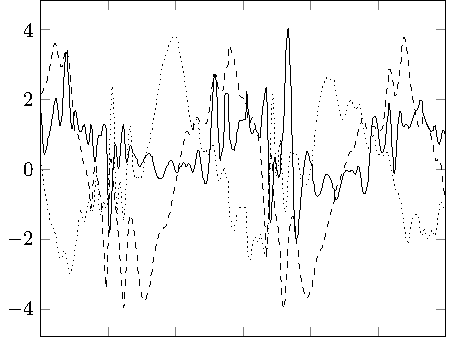
\includegraphics[width=70mm]{figures/first-exercise.pdf}}
	\subfigure[Noise]{\label{fig:first-noise}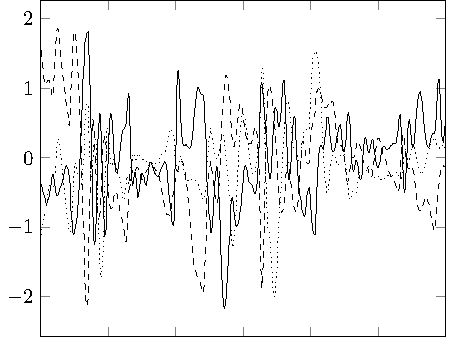
\includegraphics[width=70mm]{figures/first-noise.pdf}}
	\subfigure[Stairs]{\label{fig:first-stairs}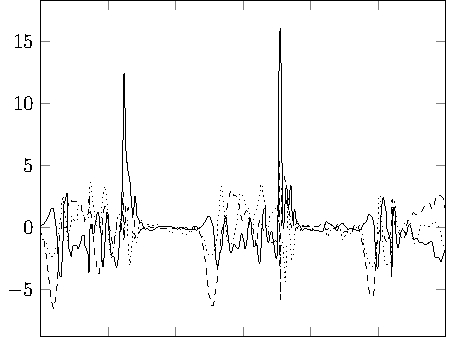
\includegraphics[width=70mm]{figures/first-stairs.pdf}}
	\subfigure[Walking]{\label{fig:first-walking}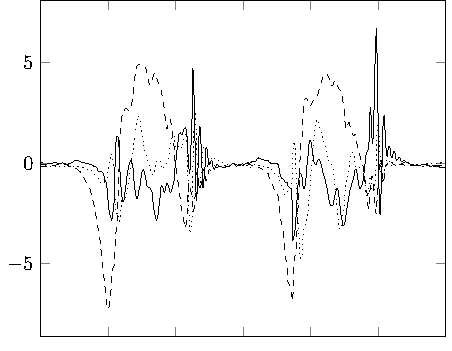
\includegraphics[width=70mm]{figures/first-walking.pdf}}
	\caption{Feasibility Assessment Data \label{fig:first-data}}
\end{figure}

%%%%%%%%%%%%%%%%%%%%%%%%%%%%%
%%% TOOLS USED / PRODUCED %%%
%%%%%%%%%%%%%%%%%%%%%%%%%%%%%
\subsection{Tools \label{sec:tools}}
Weka, a machine learning library, was used extensively for machine learning aspects. It provides a vast multitude of implemented machine learning algorithms, including various methods of evaluating the performance of these trained models.

%%%%%%%%%%%%%%%%%%%%%%%
%%% THE ARFF SCRIPT %%%
%%%%%%%%%%%%%%%%%%%%%%%
In order to produce this, it is first necessary to know the desired classification over given intervals for some time series data. This is achieved by mapping a single point of interest on some time series data to a class. This mapping is then passed to a script that takes windows centered on these points of interest and creates the corresponding \texttt{.arff}. In addition to these points of interest, the number of samples per window is also taken.

%%%%%%%%%%%%%%%%%%%%
%%% DOWNSAMPLING %%%
%%%%%%%%%%%%%%%%%%%%
Data collection is already an expensive task in terms of time consumed. It was therefore deemed infeasible to sample at multiple frequencies on top of all the variables being explored during data collection. Further to this, the device being used for data collection was rigid in terms of allowable sampling frequencies. To allow for analysis of multiple sampling frequencies at a later data, sampling was done at 200Hz, the fastest the collection device would allow. Any collected data could then be downsampled, which was achieved by taking the closest sample to $n/f$ where f is the frequency to downsample to.

%%%%%%%%%%%%%%%%%%%%%%
%%% CLASSIFICATION %%%
%%%%%%%%%%%%%%%%%%%%%%
As shown in figure \ref{fig:first-data}, activities produce periodic data that is easily manually identified. This feature of the collected data was used to in order to identify the intervals for classification. Collected data was separated at the time of collection into individual files each representing a different activity/sensor tuple, allowing for trivial manual classification.

The act of data classification occurred by viewing the plotted data and points of interest were noted. For the two exercise classes \todo{Name the classes?}, the points of interest were the peak and trough of the y-axis. For the class representing not exercise, points of interest were taken at frequent points throughout collected data files where subjects were not performing exercise, meaning that manual classification of the not exercise class was not required.

These classified points of interest were then run through a script 

%%%%%%%%%%%%%%%%%%%%%%%%%%%%%%%%%%%
%%% ASSESSING MODEL PERFORMANCE %%%
%%%%%%%%%%%%%%%%%%%%%%%%%%%%%%%%%%%
There are multiple methods of assessing the performance of a model. A simple assessment may include measuring the accuracy, although this does not take into account the probability of specific classes existing, and can therefore skew results when there are significantly more instances of a subset of classes over another subset of classes. An extreme example of this is the 0-R classifier, which will determine the most frequent class and classify all instances as this. Such a classifier is very simple, and has a severely limited utility, but as shown in \todo{figure}, a high accuracy is still possible, despite what can be considered poor performance.

By taking into account the probability of classes existing, the bias that leads to this poor metric can be eliminated. Such a statistic is the kappa statistic \todo{add cite}, which measures performance with respect to a null classifier, that is, a classifier that solely takes into account the frequencies of observed data. A kappa statistic, $\kappa < 0$  would indicate very bad performance (worse than guessing while taking into account the class frequencies). $\kappa$ increasing from 0 to 1 indicates increasing performance, with $\kappa = 1$ being a perfect classifier. The kappa statistic has therefore been used to measure the performance of later classifiers.

% Maybe remove this
In some cases, it may be important to quantify the trade-off a classifier makes between true and false positives. This can especially be the case where it is more important to detect some class over another. Achieving this can be done with a custom cost function, which is applied to the resultant confusion matrix (equation \ref{eq:cost}). From this, the average cost per instance can be computed, allowing comparisons to be drawn.

\begin{equation}
	\label{eq:cost}
	\begin{gathered}
		\text{Cost } c = \langle \mathbf{COST}, \mathbf{CONFUSION} \rangle_F \\
		\text{Where $\langle \mathbf{A}, \mathbf{B}\rangle_F$ is the Frobenius inner product between $\mathbf{A}$ and $\mathbf{B}$}
	\end{gathered}
\end{equation}

This method of performance quantification is similar to an ROC curve, except where 

Weka accepts instances in the form of an \texttt{.arff} file, this file specifies all the classes for the classifier to accept; the inputs for the classifier; and some number of instances and their actual class, if known.


%%%%%%%%%%%%%%%%%%%%%%%%%%%%%
%%% 3 CLASSES OVER JUST 2 %%%
%%%%%%%%%%%%%%%%%%%%%%%%%%%%%
The number of classes to classify was considered, as a variable parameter for the classifier. A classifier with the 2 classes \textit{exercise} \todo{Maybe s/exercise/activity/} and \textit{not exercise}, would only allow for binary classification. Depending on the classifier behaviour and the nature of the exercise in question, it may be the case that when the window of classification lies between 2 exercises, the window could be classified as either class. This unpredictable behaviour would prevent further analysis of the subject's exercise beyond how much time exercise has been detected for. \todo{Add figure}. However, by splitting the \textit{exercise} class into 2 distinct classes, such that every exercise performed will always be composed of these parts, it allows 3 classes to be used with the classifier. Such a change would allow counting of distinct exercises, by ensuring that one type of \textit{exercise} class is followed by the other type of \textit{exercise} class. This would allow the number of exercises to be counted, as well as the amount of time exercised. Further to this, the additional information may allow for heuristics to increase accuracy should the classifier ``bounce''. \todo{More on this in heuristics...} Other numbers of classes were also considered, such as some number of classes for the exercise, along with a class for each likely type of non-exercise activity. \todo{and this idea was rejected because...}

\note{What classification algorithms were trialled? What kind of results were achieved with these. Explain and discuss the workings of each algorithm / type of algorithm.}

\subsection{Multilayer Perceptrons}
A Multilayer Perceptron (MLP) is a type Neural Network, where the nodes, or perceptrons, are organised in layers. Each node accepts some number of inputs with some weight. These summation of these weighted inputs are computed and applied to some activation function, the result of which is the output of the node (equation \ref{eq:perceptron}).

\begin{equation}
\label{eq:perceptron}
\text{Output } o = activation\bigg(\sum_{i=1}^{d}{x_iw_i}\bigg) 
\end{equation}

Each perceptron affectively defines a plane in $d$-dimensional space. Instances on either side of this plane can then be classed, allowing a single perceptron to act as a simple classifier. By combining multiple perceptrons in a layer, it is possible to build up these planes in order to create more complex classifier made of these linear classifiers. The addition of layers, using previous layers are inputs allows a more complex classifier still by allowing the importance of these sub-classifiers to vary with the inputs. MLPs with enough inputs and layers can therefore replicate any function \cite{baum1988capabilities}.

\note{Finish/tidy this and wrap in figure}
\begin{tikzpicture}[shorten >=1pt,node distance=1.3cm and 3cm,on grid,auto,initial text={}] 
\node[state,initial] (i1) {$i_1$};
\node[state,initial] (i2) [below=of i1] {$i_2$}; 
\node[state,initial] (in) [below=of i2] {$i_n$}; 

\node[state] (h11) [right=of i1] {$h_{1,1}$};
\node[state] (h12) [below=of h11] {$h_{1,2}$}; 
\node[state] (h1a) [below=of h12] {$h_{1,a}$}; 

\node[state] (hb1) [right=of h11] {$h_{b,1}$};
\node[state] (hb2) [below=of hb1] {$h_{b,2}$}; 
\node[state] (hba) [below=of hb2] {$h_{b,a}$}; 

\node[state] (o) [right=of hb2] {$o$};
\path[->] 
(i1) edge node {} (h11) (i2) edge node {} (h11)
(i1) edge node {} (h12) (i2) edge node {} (h12)
(i1) edge node {} (h1a) (i2) edge node {} (h1a)
(in) edge node {} (h11) (h11) edge node {} (hb1)
(in) edge node {} (h12) (h11) edge node {} (hb2)
(in) edge node {} (h1a) (h11) edge node {} (hba)
(h12) edge node {} (hb1) (h1a) edge node {} (hb1)
(h12) edge node {} (hb2) (h1a) edge node {} (hb2)
(h12) edge node {} (hba) (h1a) edge node {} (hba)

(hb1) edge node {} (o)
(hb2) edge node {} (o)
(hba) edge node {} (o)
;
\end{tikzpicture}

\subsection{Radial Basis Function Networks}
A Radial Basis Function (RBF) network is a type of Neural Network that is composed of 2 layers, an input layer and an output layer. The activation functions for this output layer are RBFs. An RBF can be any function that is only dependent on the distance from some point. An example of a commonly used RBF is the Gaussian function.

\subsection{Instance-Based Learning}
Instance-based learning is a type of machine learning algorithm that postpones model creation until an output for a problem instance is required. Some number of labelled instances are stored in memory, and these are used to label problem instances.

Instance-based learning is advantageous over other machine learning methods in that adapting the model with new instances is trivial. This makes it attractive for simple systems where some adaptation of the model is required.

As a number of labelled instanced must be kept in memory in order to compute the model, instance-based learning methods can require large amounts of memory to classify. Additionally, any problem instances must be compared against each labelled instanced that is to be used for the model, meaning that time complexity for classification of any problem instance is linear in the number of labelled instances. This can present significant challenges when the size of the training data set become large with respect to the underlying device.

An example of instance-based learning is the k-nearest neighbours algorithm where any problem instance is compared to the k-nearest labelled instances. The class that the problem instance is most similar to is then given this classification. \todo{Reword}

\note{What issues were faced as a result of implementing a machine learning algorithm on a constrained system? How were these problems overcome? \cite{anguita2012human}}
Each machine learning algorithm comes with its own memory-processing-accuracy trade-off, 

%%%%%%%%%%%%%%%%%%%%%%%%%%%%
%%% ALGORITHM PARAMETERS %%%
%%%%%%%%%%%%%%%%%%%%%%%%%%%%
\note{Selection of the algorithm - mention hidden layers  /frequency}
There are many parameters that affect the performance of classifiers. In the case of the collected data, the sampling frequency for the kinematic sensor and the window with a number of samples over which the classifier classifies have a direct impact on the classifier's ability to perform. In the case of the model, most machine learning algorithms have some form parameters allowing their behaviour to change. 

As the MLP was 

%%%%%%%%%%%%%%%%%%%%%%%%%%
%%% USER STUDY RESULTS %%%
%%%%%%%%%%%%%%%%%%%%%%%%%%
\subsection{User Study Results}
\note{As a result of the user study, how did the results change? Note observed results due to the user study.}
The user study was performed on a number \todo{How many?} subjects, where both accelerometer and gyroscope data was collected for multiple activities.

%%%%%%%%%%%%%%%%%%%%%%%%%%%
%%% ALGORITHM SELECTION %%%
%%%%%%%%%%%%%%%%%%%%%%%%%%%
The main contenders for the algorithm were the MLP and RBF network due to high performance while having relatively low complexity, allowing them to be implemented on a constrained device without too much difficulty. Between these two algorithms, there was minimal difference in terms of 

\begin{figure}
	\centering
	\subfigure[Top-Down]{\label{fig:mlp-multi-flat}\includegraphics[width=70mm]{figures/mlp-multi-analysis-flat.pdf}}
	\subfigure[Side-On, Varying Hidden Layers]{\label{fig:mlp-multi-3d}\includegraphics[width=64mm]{figures/mlp-multi-analysis-3d.pdf}}
	%\subfigure[Varying Frequency]{\label{fig:mlp-multi-3d-2}\includegraphics[width=70mm]{figures/mlp-multi-analysis-3d-2.pdf}}
	%\subfigure[Varying Both]{\label{fig:mlp-multi-3d-3}\includegraphics[width=70mm]{figures/mlp-multi-analysis-3d-3.pdf}}
	\caption{MLP Parameter Performance Surface Plot \label{fig:mlp-multi}}
\end{figure}

\begin{figure}
	\includegraphics[width=\linewidth]{subject-fold-results.pdf}
	\caption{Subject Performance with Different Sensors and Algorithms \label{fig:subfold}}
\end{figure}

%%%%%%%%%%%%%%%%%%%%%%%%%%%%%%%%%%%
%%% WHY CROSS-VALIDATION IS BAD %%%
%%%%%%%%%%%%%%%%%%%%%%%%%%%%%%%%%%%
To evaluate the models on the user study data, cross-validation was considered, as this would allow training on some set of data and then testing on another set previously unseen to the model, although this would have the slightly undesirable effect of mixing data from subjects, whereas in practice, the device will be trained on a set of subjects and used by a subject not in that set. To replicate this kind of behaviour, a similar method to cross-validation was used, where the model was trained on all subjects, except for one. This one excluded subject was then tested on. This method is then repeated for all subjects. This subject-fold cross-validation method is also beneficial in allowing conclusions to be drawn about subject performance in relation to other subjects.

A noteworthy observation about the results was that the performance of the algorithm was initially poor, by any measure, after the first day data collection, giving just 5 \todo{Really?} subjects to model against. However, as the number of subjects increased, so did the performance of the system. This would indicate that the algorithm was overfitting on subjects, and that the introduction of more subjects was able to at least in part negate this overfitting.

\note{What parameters are there and how did they affect the accuracy of the system?}
	\appendix
	\chapter{Risk Assessment}

The project's risk assessment is shown on the following two pages, ordered from highest priority to lowest. The
first two risks did materialise for this team, however the
planned mitigation was appropriate so there were no significant issues caused by these.

\begin{landscape}
\begin{table}
\begin{tabular}{ | m{3cm} | m{6.5cm} | m{2cm} | m{1.5cm} | m{1.5cm} | m{7cm} | } 
  \hline
  Risk & Description & Likelihood & Impact & Priority & Mitigation \\
  \hline

  Developer Health &
  Ongoing health issues with one team member may disrupt their ability to work &
  0.8 & 0.6 & 0.48 &
  . \\
  \hline

  Ethical Approval Delays &
  Issues receiving ethical approval may delay the date at which initial collection can be done, which would in turn delay the development schedule. &
  0.6 & 0.6 & 0.36 &
  Plan to complete the ethical approval request early in the project. Ensure the development schedule does not rely on the movement data from the very beginning. \\
  \hline
 
  Unable to scale algorithm &
  The system we have been given does not allow division or floating point. It may not be possible to reduce an algorithm to these constraints without prohibitively low running time &
  0.5 & 0.7 & 0.35 &
  Use this constraint when deciding an optimum algorithm: where possible, choose methods which require less computation and, specifically, fewer operations relying on complex mathematical operations which require accurate floating point or division. \\
  \hline

  Code does not fit on device &
  When compiling the code, its size may exceed the maximum of 8KB meaning it will not fit onto the device. This may happen because too many libraries are required or the algorithm itself is too large &
  0.4 & 0.8 & 0.32 &
  Use this constraint when deciding an optimum algorithm: where possible, choose lower sampling frequencies as these require less weights \\
  \hline

  Not able to recognise exercises &
  The possibility that no algorithm can be discovered or created to distinguish exercise from non-exercise &
  0.3 & 0.9 & 0.27 &
  Use Weka, a well known and well tested, tool designed to bulk test multiple existing machine learning algorithms \\
  \hline
\end{tabular}
\label{table:risk-1}
\caption{Risk Assessment}
\end{table}

\begin{table}
\begin{tabular}{ | m{3cm} | m{6.5cm} | m{2cm} | m{1.5cm} | m{1.5cm} | m{7cm} | } 
  \hline
  Risk & Description & Likelihood & Impact & Priority & Mitigation \\
  \hline

  Loss of work &
  Technical, physical or human issues may lead to loss of work or data, which will delay progress
  & 0.3 & 0.9 & 0.27 &
  All code kept under Git version control, where this is not under licence it will be backed up to GitHub. Repositories which include non-publishable code will be backed up to a personal git server of one of the team members. All documents written using LaTeX, which will also be kept under version control, or Google Documents. \\
  \hline

  Unable to perform second participant study  &
  There may not be enough time to test the prototype on a large selection of participants to measure its effectiveness  &
  0.8 & 0.2 & 0.16 &
  We can perform the tests on ourselves which should give sufficient indication on how well the prototype performs. \\
  \hline
  
  FPGA &
  The FPGA is a complex device - if we are unable to obtain or understand the relevant documentation, it will be difficult to complete the required verilog &
  0.3 & 0.5 & 0.15 &
  Ask ARM for the required documentation and maintain contact in case of issues. \\
  \hline

  mBed clock speed &
  The mBed's specification states that it may have an error on its clock speed, making measurements difficult &
  0.1 & 0.1 & 0.01 &
  Test clock speeds under various conditions to see the impact. Also develop on the FPGA which does not have this issue. \\
  \hline

  Code cannot be compiled &
  Issues with library compatibilities or compiler limitations may cause problems when compiling our code for the device &
  0.1 & 0.8 & 0.08 &
  Use ARM's provided compiler, which is well supported and relies on common libraries. \\
  \hline
 
\end{tabular}
\label{table:risk-2}
\caption{Risk Assessment Cont.}
\end{table}
\end{landscape}

	%
	\backmatter
	\bibliographystyle{../../bibtex/bst/ecsdocs/ecs}
	\bibliography{bib}
\end{document}
%% ----------------------------------------------------------------
